% Options for packages loaded elsewhere
% Options for packages loaded elsewhere
\PassOptionsToPackage{unicode}{hyperref}
\PassOptionsToPackage{hyphens}{url}
\PassOptionsToPackage{dvipsnames,svgnames,x11names}{xcolor}
%
\documentclass[
  a4paper,
  DIV=11,
  numbers=noendperiod]{scrartcl}
\usepackage{xcolor}
\usepackage{amsmath,amssymb}
\setcounter{secnumdepth}{-\maxdimen} % remove section numbering
\usepackage{iftex}
\ifPDFTeX
  \usepackage[T1]{fontenc}
  \usepackage[utf8]{inputenc}
  \usepackage{textcomp} % provide euro and other symbols
\else % if luatex or xetex
  \usepackage{unicode-math} % this also loads fontspec
  \defaultfontfeatures{Scale=MatchLowercase}
  \defaultfontfeatures[\rmfamily]{Ligatures=TeX,Scale=1}
\fi
\usepackage{lmodern}
\ifPDFTeX\else
  % xetex/luatex font selection
\fi
% Use upquote if available, for straight quotes in verbatim environments
\IfFileExists{upquote.sty}{\usepackage{upquote}}{}
\IfFileExists{microtype.sty}{% use microtype if available
  \usepackage[]{microtype}
  \UseMicrotypeSet[protrusion]{basicmath} % disable protrusion for tt fonts
}{}
\makeatletter
\@ifundefined{KOMAClassName}{% if non-KOMA class
  \IfFileExists{parskip.sty}{%
    \usepackage{parskip}
  }{% else
    \setlength{\parindent}{0pt}
    \setlength{\parskip}{6pt plus 2pt minus 1pt}}
}{% if KOMA class
  \KOMAoptions{parskip=half}}
\makeatother
% Make \paragraph and \subparagraph free-standing
\makeatletter
\ifx\paragraph\undefined\else
  \let\oldparagraph\paragraph
  \renewcommand{\paragraph}{
    \@ifstar
      \xxxParagraphStar
      \xxxParagraphNoStar
  }
  \newcommand{\xxxParagraphStar}[1]{\oldparagraph*{#1}\mbox{}}
  \newcommand{\xxxParagraphNoStar}[1]{\oldparagraph{#1}\mbox{}}
\fi
\ifx\subparagraph\undefined\else
  \let\oldsubparagraph\subparagraph
  \renewcommand{\subparagraph}{
    \@ifstar
      \xxxSubParagraphStar
      \xxxSubParagraphNoStar
  }
  \newcommand{\xxxSubParagraphStar}[1]{\oldsubparagraph*{#1}\mbox{}}
  \newcommand{\xxxSubParagraphNoStar}[1]{\oldsubparagraph{#1}\mbox{}}
\fi
\makeatother

\usepackage{color}
\usepackage{fancyvrb}
\newcommand{\VerbBar}{|}
\newcommand{\VERB}{\Verb[commandchars=\\\{\}]}
\DefineVerbatimEnvironment{Highlighting}{Verbatim}{commandchars=\\\{\}}
% Add ',fontsize=\small' for more characters per line
\usepackage{framed}
\definecolor{shadecolor}{RGB}{241,243,245}
\newenvironment{Shaded}{\begin{snugshade}}{\end{snugshade}}
\newcommand{\AlertTok}[1]{\textcolor[rgb]{0.68,0.00,0.00}{#1}}
\newcommand{\AnnotationTok}[1]{\textcolor[rgb]{0.37,0.37,0.37}{#1}}
\newcommand{\AttributeTok}[1]{\textcolor[rgb]{0.40,0.45,0.13}{#1}}
\newcommand{\BaseNTok}[1]{\textcolor[rgb]{0.68,0.00,0.00}{#1}}
\newcommand{\BuiltInTok}[1]{\textcolor[rgb]{0.00,0.23,0.31}{#1}}
\newcommand{\CharTok}[1]{\textcolor[rgb]{0.13,0.47,0.30}{#1}}
\newcommand{\CommentTok}[1]{\textcolor[rgb]{0.37,0.37,0.37}{#1}}
\newcommand{\CommentVarTok}[1]{\textcolor[rgb]{0.37,0.37,0.37}{\textit{#1}}}
\newcommand{\ConstantTok}[1]{\textcolor[rgb]{0.56,0.35,0.01}{#1}}
\newcommand{\ControlFlowTok}[1]{\textcolor[rgb]{0.00,0.23,0.31}{\textbf{#1}}}
\newcommand{\DataTypeTok}[1]{\textcolor[rgb]{0.68,0.00,0.00}{#1}}
\newcommand{\DecValTok}[1]{\textcolor[rgb]{0.68,0.00,0.00}{#1}}
\newcommand{\DocumentationTok}[1]{\textcolor[rgb]{0.37,0.37,0.37}{\textit{#1}}}
\newcommand{\ErrorTok}[1]{\textcolor[rgb]{0.68,0.00,0.00}{#1}}
\newcommand{\ExtensionTok}[1]{\textcolor[rgb]{0.00,0.23,0.31}{#1}}
\newcommand{\FloatTok}[1]{\textcolor[rgb]{0.68,0.00,0.00}{#1}}
\newcommand{\FunctionTok}[1]{\textcolor[rgb]{0.28,0.35,0.67}{#1}}
\newcommand{\ImportTok}[1]{\textcolor[rgb]{0.00,0.46,0.62}{#1}}
\newcommand{\InformationTok}[1]{\textcolor[rgb]{0.37,0.37,0.37}{#1}}
\newcommand{\KeywordTok}[1]{\textcolor[rgb]{0.00,0.23,0.31}{\textbf{#1}}}
\newcommand{\NormalTok}[1]{\textcolor[rgb]{0.00,0.23,0.31}{#1}}
\newcommand{\OperatorTok}[1]{\textcolor[rgb]{0.37,0.37,0.37}{#1}}
\newcommand{\OtherTok}[1]{\textcolor[rgb]{0.00,0.23,0.31}{#1}}
\newcommand{\PreprocessorTok}[1]{\textcolor[rgb]{0.68,0.00,0.00}{#1}}
\newcommand{\RegionMarkerTok}[1]{\textcolor[rgb]{0.00,0.23,0.31}{#1}}
\newcommand{\SpecialCharTok}[1]{\textcolor[rgb]{0.37,0.37,0.37}{#1}}
\newcommand{\SpecialStringTok}[1]{\textcolor[rgb]{0.13,0.47,0.30}{#1}}
\newcommand{\StringTok}[1]{\textcolor[rgb]{0.13,0.47,0.30}{#1}}
\newcommand{\VariableTok}[1]{\textcolor[rgb]{0.07,0.07,0.07}{#1}}
\newcommand{\VerbatimStringTok}[1]{\textcolor[rgb]{0.13,0.47,0.30}{#1}}
\newcommand{\WarningTok}[1]{\textcolor[rgb]{0.37,0.37,0.37}{\textit{#1}}}

\usepackage{longtable,booktabs,array}
\usepackage{calc} % for calculating minipage widths
% Correct order of tables after \paragraph or \subparagraph
\usepackage{etoolbox}
\makeatletter
\patchcmd\longtable{\par}{\if@noskipsec\mbox{}\fi\par}{}{}
\makeatother
% Allow footnotes in longtable head/foot
\IfFileExists{footnotehyper.sty}{\usepackage{footnotehyper}}{\usepackage{footnote}}
\makesavenoteenv{longtable}
\usepackage{graphicx}
\makeatletter
\newsavebox\pandoc@box
\newcommand*\pandocbounded[1]{% scales image to fit in text height/width
  \sbox\pandoc@box{#1}%
  \Gscale@div\@tempa{\textheight}{\dimexpr\ht\pandoc@box+\dp\pandoc@box\relax}%
  \Gscale@div\@tempb{\linewidth}{\wd\pandoc@box}%
  \ifdim\@tempb\p@<\@tempa\p@\let\@tempa\@tempb\fi% select the smaller of both
  \ifdim\@tempa\p@<\p@\scalebox{\@tempa}{\usebox\pandoc@box}%
  \else\usebox{\pandoc@box}%
  \fi%
}
% Set default figure placement to htbp
\def\fps@figure{htbp}
\makeatother





\setlength{\emergencystretch}{3em} % prevent overfull lines

\providecommand{\tightlist}{%
  \setlength{\itemsep}{0pt}\setlength{\parskip}{0pt}}



 


\KOMAoption{captions}{tableheading}
\makeatletter
\@ifpackageloaded{caption}{}{\usepackage{caption}}
\AtBeginDocument{%
\ifdefined\contentsname
  \renewcommand*\contentsname{Table of contents}
\else
  \newcommand\contentsname{Table of contents}
\fi
\ifdefined\listfigurename
  \renewcommand*\listfigurename{List of Figures}
\else
  \newcommand\listfigurename{List of Figures}
\fi
\ifdefined\listtablename
  \renewcommand*\listtablename{List of Tables}
\else
  \newcommand\listtablename{List of Tables}
\fi
\ifdefined\figurename
  \renewcommand*\figurename{Figure}
\else
  \newcommand\figurename{Figure}
\fi
\ifdefined\tablename
  \renewcommand*\tablename{Table}
\else
  \newcommand\tablename{Table}
\fi
}
\@ifpackageloaded{float}{}{\usepackage{float}}
\floatstyle{ruled}
\@ifundefined{c@chapter}{\newfloat{codelisting}{h}{lop}}{\newfloat{codelisting}{h}{lop}[chapter]}
\floatname{codelisting}{Listing}
\newcommand*\listoflistings{\listof{codelisting}{List of Listings}}
\makeatother
\makeatletter
\makeatother
\makeatletter
\@ifpackageloaded{caption}{}{\usepackage{caption}}
\@ifpackageloaded{subcaption}{}{\usepackage{subcaption}}
\makeatother
\usepackage{bookmark}
\IfFileExists{xurl.sty}{\usepackage{xurl}}{} % add URL line breaks if available
\urlstyle{same}
\hypersetup{
  pdftitle={Week 5 Tutorial},
  colorlinks=true,
  linkcolor={blue},
  filecolor={Maroon},
  citecolor={Blue},
  urlcolor={Blue},
  pdfcreator={LaTeX via pandoc}}


\title{Week 5 Tutorial}
\author{}
\date{}
\begin{document}
\maketitle


\definecolor{awesome}{rgb}{1.0,0.13,0.32}
\definecolor{bondiblue}{rgb}{0.0,0.58,0.71}

\subsubsection{Introduction}\label{introduction}

This tutorial will help you familiarize yourself with optimal portfolio
selection. We will use the \textbf{Solver} add-in from Microsoft Excel,
so please:

\begin{itemize}
\tightlist
\item
  open the \textcolor{blue}{\textbf{W5Q1Solver.xlsx}} file from Moodle.
\item
  install Solver
\end{itemize}

\subsubsection{Question 1}\label{question-1}

Assume three risky assets, namely Microsoft (M), Nordstrom (N) and
Starbucks (S). Let \(r_{i}\) denote the return on asset \(i\) where
\(i=M,N,S\). The following information is given for these assets:

\[ \begin{tabular}{|l|c|c|c|c|}
\hline
Stock $i$ & $\mu _{i}$ & $\sigma _{i}$ & Pairs ($i,j$) & $\sigma _{ij}$ \\ 
\hline
M (Microsoft) & 0.0427 & 0.1000 & (M,N) & 0.0018 \\ \hline
N (Nordstrom) & 0.0015 & 0.1044 & (M,S) & 0.0011 \\ \hline
S (Starbucks) & 0.0285 & 0.1411 & (N,S) & 0.0026 \\ \hline
\end{tabular} \]

where \(\mu _{i},\) \(\sigma _{i}\) and \(\sigma _{ij}\) denote expected
returns, standard deviations and covariances for each asset,
respectively.

\begin{enumerate}
\def\labelenumi{\arabic{enumi}.}
\item
  Construct a \(3\times 1\) vector, \(\boldsymbol{\mu }\), containing
  the expected returns of these three assets. Similarly, construct the
  \(3\times 3\) variance-covariance matrix, \(\boldsymbol{\Sigma }\),
  associated with the performance of these assets based on the
  information provided (do this in the \textbf{W5Q1Solver.xlsx} file).
\item
  Consider a portfolio, P, that consists of assets M,N,S, with return
  given by: \[r_{P}=w_{M}r_{M}+w_{N}r_{N}+w_{S}r_{S},\] where
  \(w_{M},w_{N},w_{S}\) are the (non-negative) weights assigned to each
  of the assets, such that \(w_{M}+w_{N}+w_{S}=1\). Using matrix
  notation write the analytical expressions for portfolio expected
  return, \(\mu _{P}\), and portfolio variance, \(\sigma _{P}^{2}\).
\item
  Find the numerical solution to this optimization problem in Excel
  using the information provided in the table above (make use of the
  Excel add-in ``Solver'').
\item
  Find the analytic solution to the following optimization problem
  \[\min_{w_{M},w_{N},w_{S}}\sigma _{P}^{2}\text{, such that }w_{M}+w_{N}+w_{S}=1,\]
  using the Lagrange multiplier method. {[}not required{]}
\item
  Using the analytical formula for the vector of optimal weights in part
  4, compute the optimal weights assigned to the Global Minimum Variance
  portfolio.
\end{enumerate}

\textcolor{awesome}{\textbf{Use the tab named 'Analytical' in the Excel file (as in Part 3) and matrix multiplication in Excel.}}

\subsection{Question 2}\label{question-2}

Consider stock prices for Microsoft (MSFT) and Walmart (WMT) from 1990
to 2024. The stock prices can be found in the file
\textcolor{blue}{\textbf{msft\_wmt.wf1}} in the tutorial folder. Use
these data to answer the following questions.

\begin{enumerate}
\def\labelenumi{\arabic{enumi}.}
\tightlist
\item
  Compute the log-returns on Microsoft and Walmart at the monthly
  frequency.
\end{enumerate}

\textcolor{awesome}{\textbf{Download the "msft\_wmt.xslx" file from Moodle into your project and run the code below.}}

\textcolor{awesome}{First we need to load the \textbf{xts} library and create better dates (the original date format is incompatible with xts). We will look at what we have and plot the data.}

\begin{Shaded}
\begin{Highlighting}[]
\FunctionTok{library}\NormalTok{(xts)}
\end{Highlighting}
\end{Shaded}

\begin{verbatim}
Warning: package 'xts' was built under R version 4.5.3
\end{verbatim}

\begin{verbatim}
Loading required package: zoo
\end{verbatim}

\begin{verbatim}
Warning: package 'zoo' was built under R version 4.5.3
\end{verbatim}

\begin{verbatim}

Attaching package: 'zoo'
\end{verbatim}

\begin{verbatim}
The following objects are masked from 'package:base':

    as.Date, as.Date.numeric
\end{verbatim}

\begin{Shaded}
\begin{Highlighting}[]
\NormalTok{mw\_df }\OtherTok{\textless{}{-}}\NormalTok{ readxl}\SpecialCharTok{::}\FunctionTok{read\_excel}\NormalTok{(}\StringTok{"msft\_wmt.xlsx"}\NormalTok{)   }\CommentTok{\# \textless{}{-}{-} change filename}

\CommentTok{\# ignore the date column}
\NormalTok{mw\_df }\OtherTok{=}\NormalTok{ mw\_df[,}\SpecialCharTok{{-}}\DecValTok{1}\NormalTok{]}

\CommentTok{\# Jan 1990 to March 2024}
\CommentTok{\# create an xts object, but first create the date. }
\NormalTok{idx }\OtherTok{\textless{}{-}} \FunctionTok{seq}\NormalTok{(}\AttributeTok{from =} \FunctionTok{as.Date}\NormalTok{(}\StringTok{"1990{-}01{-}01"}\NormalTok{), }\AttributeTok{by =} \StringTok{"month"}\NormalTok{, }\AttributeTok{length.out =} \FunctionTok{nrow}\NormalTok{(mw\_df))}
\NormalTok{prices.xts }\OtherTok{\textless{}{-}} \FunctionTok{xts}\NormalTok{(mw\_df, }\AttributeTok{order.by =}\NormalTok{ idx)}

\CommentTok{\# just display month{-}year without date}
\FunctionTok{index}\NormalTok{(prices.xts) }\OtherTok{\textless{}{-}} \FunctionTok{as.yearmon}\NormalTok{(}\FunctionTok{index}\NormalTok{(prices.xts))  }
\FunctionTok{head}\NormalTok{(prices.xts)}
\end{Highlighting}
\end{Shaded}

\begin{verbatim}
             MSFT      WMT
Jan 1990 0.642361 1.093507
Feb 1990 0.685764 1.128781
Mar 1990 0.769097 1.212157
Apr 1990 0.805556 1.274974
May 1990 1.013889 1.448397
Jun 1990 1.055556 1.602550
\end{verbatim}

\begin{Shaded}
\begin{Highlighting}[]
\FunctionTok{plot}\NormalTok{(prices.xts, }\AttributeTok{legend.loc =} \StringTok{"topleft"}\NormalTok{, }\AttributeTok{main =} \StringTok{"Prices"}\NormalTok{)}
\end{Highlighting}
\end{Shaded}

\pandocbounded{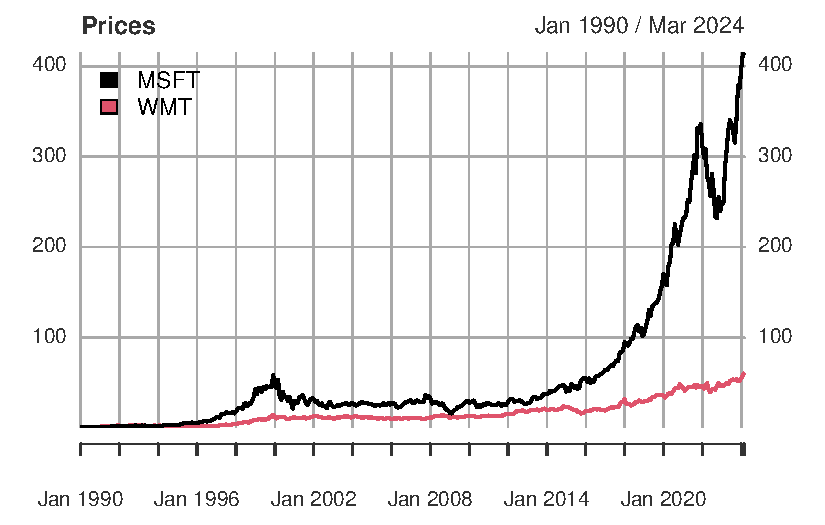
\includegraphics[keepaspectratio]{Tutorial-Week-5pdfr_files/figure-pdf/unnamed-chunk-1-1.pdf}}

\textcolor{awesome}{Now, as usual, we calculate log-returns. This time we will do both at a time and create two columns.}

\begin{Shaded}
\begin{Highlighting}[]
\CommentTok{\# log return for both msft and wmt}
\NormalTok{logret.xts }\OtherTok{\textless{}{-}} \FunctionTok{diff}\NormalTok{(}\FunctionTok{log}\NormalTok{(prices.xts)) }
\NormalTok{logret.xts }\OtherTok{\textless{}{-}} \FunctionTok{na.omit}\NormalTok{(logret.xts)   }\CommentTok{\# removes the first NA created by diff()}
\FunctionTok{colnames}\NormalTok{(logret.xts) }\OtherTok{\textless{}{-}} \FunctionTok{c}\NormalTok{(}\StringTok{"msft"}\NormalTok{, }\StringTok{"wmt"}\NormalTok{)  }\CommentTok{\# name the column}
\end{Highlighting}
\end{Shaded}

\begin{enumerate}
\def\labelenumi{\arabic{enumi}.}
\setcounter{enumi}{1}
\tightlist
\item
  Compute the sample variance-covariance matrix of returns for these two
  stocks.
\end{enumerate}

\textcolor{awesome}{Since we have 2 columns of data, we have a simple formula to get the sample var-cov matrix.}

\begin{enumerate}
\def\labelenumi{\arabic{enumi}.}
\setcounter{enumi}{2}
\tightlist
\item
  Estimate the regression model
\end{enumerate}

\[r_{wal,t}=\beta _{0}+\beta _{1}\left( r_{wal,t}-r_{mic,t}\right) +\epsilon_{t},\]

where \(\epsilon _{t}\) is a disturbance term. Interpret the estimate of
\(\beta _{1}\).

\textcolor{awesome}{We can use logret.xts directly. We will create a new variable for the difference - msopt to make the output cleaner. We could use the I(.) function to create the difference directly in the lm(.) function, but the output is messy.}

\begin{Shaded}
\begin{Highlighting}[]
\NormalTok{msopt }\OtherTok{\textless{}{-}}\NormalTok{ logret.xts}\SpecialCharTok{$}\NormalTok{wmt}\SpecialCharTok{{-}}\NormalTok{logret.xts}\SpecialCharTok{$}\NormalTok{msft}

\NormalTok{minvar }\OtherTok{\textless{}{-}} \FunctionTok{lm}\NormalTok{(logret.xts}\SpecialCharTok{$}\NormalTok{wmt }\SpecialCharTok{\textasciitilde{}}\NormalTok{ msopt)}
\FunctionTok{summary}\NormalTok{(minvar)}
\end{Highlighting}
\end{Shaded}

\begin{verbatim}

Call:
lm(formula = logret.xts$wmt ~ msopt)

Residuals:
      Min        1Q    Median        3Q       Max 
-0.227714 -0.034376 -0.000255  0.032647  0.189722 

Coefficients:
            Estimate Std. Error t value Pr(>|t|)    
(Intercept) 0.011546   0.002769   4.169 3.74e-05 ***
msopt       0.289473   0.030860   9.380  < 2e-16 ***
---
Signif. codes:  0 '***' 0.001 '**' 0.01 '*' 0.05 '.' 0.1 ' ' 1

Residual standard error: 0.05595 on 408 degrees of freedom
Multiple R-squared:  0.1774,    Adjusted R-squared:  0.1754 
F-statistic: 87.99 on 1 and 408 DF,  p-value: < 2.2e-16
\end{verbatim}

\begin{enumerate}
\def\labelenumi{\arabic{enumi}.}
\setcounter{enumi}{4}
\tightlist
\item
  Using the regression results from the previous question, construct a
  hypothesis test that an equally weighted portfolio would result in a
  minimum variance portfolio
\end{enumerate}

\[H_{0}:\beta _{1}=0.5\text{ v.s. }H_{0}:\beta _{1}\neq 0.5.\]

\textcolor{awesome}{\textbf{NOTE: the calculated t-value and the p-value from the regresssion output is based upon testing if $\beta_1=0$ against $\beta_1\neq0$. This means that we have to calcuate the t-value manually, as well as the p-value.}}

\textcolor{awesome}{We test $H_0:\mu=0.5$ against $H_1:\mu\neq0.5$. The test statistic is $t=(\hat{\beta_1}-0.5)/s.e.(\hat{\beta_1})\sim t_{408}$ under $H_0$. The calculated \textit{t}-statistic is $t=(0.289473-0.5)/0.030860)$. The code below does this in R - you must fill in some gaps and set eval = TRUE.}

\begin{Shaded}
\begin{Highlighting}[]
\CommentTok{\# Find the calculate t{-}value}

\NormalTok{bhat  }\OtherTok{\textless{}{-}} \FunctionTok{coef}\NormalTok{(minvar)[}\StringTok{"msopt"}\NormalTok{]}
\NormalTok{se }\OtherTok{\textless{}{-}} \FunctionTok{summary}\NormalTok{(minvar)}\SpecialCharTok{$}\NormalTok{coefficients[}\StringTok{"msopt"}\NormalTok{, }\StringTok{"Std. Error"}\NormalTok{]}


\NormalTok{t\_calc }\OtherTok{\textless{}{-}}\NormalTok{ ???}


\FunctionTok{c}\NormalTok{(}\StringTok{"t{-}calc"}\NormalTok{, }\FunctionTok{round}\NormalTok{(t\_calc, }\DecValTok{3}\NormalTok{))}
\end{Highlighting}
\end{Shaded}

\begin{Shaded}
\begin{Highlighting}[]
\CommentTok{\# Find the p{-}value}
\CommentTok{\# degrees of freedom = n{-}2}

\NormalTok{dfr }\OtherTok{\textless{}{-}} \FunctionTok{nobs}\NormalTok{(minvar) }\SpecialCharTok{{-}} \DecValTok{2}

\CommentTok{\# p{-}value {-} find area in tails from t\_calc in a t dist with n{-}1 df }

\CommentTok{\# pt gives are to the LEFT, so we need to always use the negative t\_calc}

\CommentTok{\# {-}abs(.) will always be negative, regardless of the sign of t\_calc}

\NormalTok{p\_val  }\OtherTok{\textless{}{-}} \FunctionTok{round}\NormalTok{(???, dfr),}\DecValTok{3}\ErrorTok{)} 

\FunctionTok{c}\NormalTok{(}\StringTok{"p{-}value"}\NormalTok{, p\_val)}
\end{Highlighting}
\end{Shaded}





\end{document}
